%for a more compact document, add the option openany to avoid
%starting all chapters on odd numbered pages
\documentclass[12pt]{cmuthesis}

% This is a template for a CMU thesis.  It is 18 pages without any content :-)
% The source for this is pulled from a variety of sources and people.
% Here's a partial list of people who may or may have not contributed:
%
%        bnoble   = Brian Noble
%        caruana  = Rich Caruana
%        colohan  = Chris Colohan
%        comar    = Cyrus Omar
%        jab      = Justin Boyan
%        josullvn = Joseph O'Sullivan
%        jrs      = Jonathan Shewchuk
%        kosak    = Corey Kosak
%        mjz      = Matt Zekauskas (mattz@cs)
%        pdinda   = Peter Dinda
%        pfr      = Patrick Riley
%        dkoes = David Koes (me)

% My main contribution is putting everything into a single class files and small
% template since I prefer this to some complicated sprawling directory tree with
% makefiles.

% some useful packages
\usepackage{times}
\usepackage{fullpage}
\usepackage{graphicx}
\usepackage{amsmath}
\usepackage[numbers,sort]{natbib}
\usepackage[backref,pageanchor=true,plainpages=false, pdfpagelabels, bookmarks,bookmarksnumbered,
%pdfborder=0 0 0,  %removes outlines around hyper links in online display
]{hyperref}
\usepackage{subcaption}

\usepackage[capitalize,noabbrev,nameinlink]{cleveref}
\usepackage{float}
\usepackage[scaled]{inconsolata}

\captionsetup{labelfont=bf}
% \captionsetup{font=small}
\captionsetup{labelfont=bf}
\captionsetup{textfont={}}
%\captionsetup[subfloat]{font=small}
%\captionsetup[subfloat]{farskip=5pt}
%\captionsetup[subfloat]{captionskip=1pt}

\DeclareUnicodeCharacter{0097}{~}


% Approximately 1" margins, more space on binding side
%\usepackage[letterpaper,twoside,vscale=.8,hscale=.75,nomarginpar]{geometry}
%for general printing (not binding)
\usepackage[letterpaper,twoside,vscale=.8,hscale=.75,nomarginpar,hmarginratio=1:1]{geometry}

% Provides a draft mark at the top of the document. 
\draftstamp{\today}{DRAFT}

\begin {document} 
\frontmatter

%initialize page style, so contents come out right (see bot) -mjz
\pagestyle{empty}

\title{ %% {\it \huge Thesis Proposal}\\
{\bf Log Replay for Code Generation in OLTP Systems}}
\author{Tianlei Pan}
\date{June}
\Year{2021}
\trnumber{}

\committee{
Andy Pavlo, Chair \\
Wenting Ye \\
}

\support{}
\disclaimer{}

% copyright notice generated automatically from Year and author.
% permission added if \permission{} given.

\keywords{Code Generation, Log Replay, Recovery, Query Compilation}

\maketitle

\begin{dedication}
\end{dedication}

\pagestyle{plain} % for toc, was empty

%% Obviously, it's probably a good idea to break the various sections of your thesis
%% into different files and input them into this file...

\begin{abstract}
Instead of interpreting log records, we are extending our query code generation engine to create custom programs to replay log records. We will also be exploring for different optimization techniques to improve the recovery speed of recovery with code generation.
\end{abstract}

\begin{acknowledgments}
yes
\end{acknowledgments}



\tableofcontents
\listoffigures
\listoftables

\mainmatter

%% Double space document for easy review:
%\renewcommand{\baselinestretch}{1.66}\normalsize

% The other requirements Catherine has:
%
%  - avoid large margins.  She wants the thesis to use fewer pages, 
%    especially if it requires colour printing.
%
%  - The thesis should be formatted for double-sided printing.  This
%    means that all chapters, acknowledgements, table of contents, etc.
%    should start on odd numbered (right facing) pages.
%
%  - You need to use the department standard tech report title page.  I
%    have tried to ensure that the title page here conforms to this
%    standard.
%
%  - Use a nice serif font, such as Times Roman.  Sans serif looks bad.
%
% Other than that, just make it look good...


\chapter{Introduction}
A \textit{database management system (DBMS)} is a software that is responsible for storing data, analyzing data, and interacting with applications. Depending on the use case, a DBMS can be designed to focus more on either capturing data, or analyzing data. \textit{On-line Analytical Processing (OLAP)} applications focus on reading, analyzing and aggregating cold data that is less likely to be modified. On the other hand, \textit{On-line Transaction Processing (OLTP)} applications work with write-heavy transactions that modify the database frequently.

Consequently, recovery and durability in OLTP applications are more of a pressing issue compared to OLAP systems. Naive or manual backups are usually sufficient for read-only OLAP applications. However, since OLTP databases are being updated by transactions constantly, naive backups will either cause the database to lose significant amount of data, or fail to preserve the \textit{ACID (atomicity, consistency, isolation, and durability)} properties of a DBMS. This requires OLTP applications to develop specialized recovery mechanism to handle these problems. \textit{Write-ahead logging (WAL)} is currently the most widely adopted recovery mechanisms for OLTP applications that preserves ACID properties.

In addition, OLTP systems also require specialized algorithms and implementations to execute write transactions. Query compilation is an important optimization technique used in OLTP systems to greatly reduce the number of instructions that need to be executed. A DBMS uses a processing model (e.g. Iterator, Vectorization, Materialization) to determine how the DBMS executes a query plan. The processing model is responsible for translating a query into an intermediate expression. The execution engine then breaks down the expression into various tasks for execution. To speed up this process, the DBMS can use an optimization technique known as \textit{Query Compilation}. Query compilation requires the DBMS to generate specialized code for execution tasks to increase execution throughput. These specialized code are often created using an off-shelf compiler into a C/C++ program that implements the functionality of a certain query. For instance, HyPer \cite{hyper_llvm} uses the LLVM compiler framework to translate queries into machine code.

While query compilation has proved successful in increasing the efficiency of a DBMS, it comes with several drawbacks. Implementing a query compilation system can be quite an ordeal. It requires additional knowledge of compiler systems (e.g. LLVM) and huge amounts of engineering work to translate different execution tasks. Moreover, the DBMS also need to modify other components to accommodate with an execution engine reliant on query compilation.

One of such components is the recovery system. The structure of log records are vastly different from query plans. Therefore, to implement a recovery system in a query compilation environment, the DBMS would need to implement an additional execution engine to interpret the log records. Instead, we propose a system design that will extend the query execution engine to create custom programs for replaying log records.

\chapter{Background}
\section{Log Replay}
Database recovery systems are responsible for preserving the ACID principles of a DBMS in case of failure. Early recovery systems assume that there is no non-volatile memory. Mention Tandem here ($https://link.springer.com/chapter/10.1007/3-540-51085-0_43$). Modern DBMS can utilize a much larger memory. This allows logging protocols to be simplified (e.g. tracking dirty pages is no longer required). A modern recovery system consists of two parts: logging and recovery.

Logging is the action of storing transactional information on disk. These information are stored in a special data structure called a \textit{log record}. A log record can either contain physical information (e.g. changes made to a specific physical address) or higher-level information (e.g. user-input query). Mention MSSQL (time-travel table).

Recovery is the action of restoring the database system into a consistent state. If available, the DBMS first attempts to restore its previously recorded checkpoint. The database then initiates the log replay process that goes through every log record stored since that checkpoint. SiLO (checkpoint).

Describe how log replay works in Noisepage. (Big Picture)
Logging: Transactions are logged prior to commit.
Recovery: Independent recovery thread that loops over all the log records. The log record is either a redo record or a delete record. The contents of the record are then interpreted into either a staged write or delete. Initialization of catalog is hard-coded.

\section{Query Compilation}
part for Talk about query compilation / code generation. Mention Efficiently Compiling Efficient Query Plans
\begin{figure}[H]
\centering
\begin{subfigure}{.5\textwidth}
 \centering
 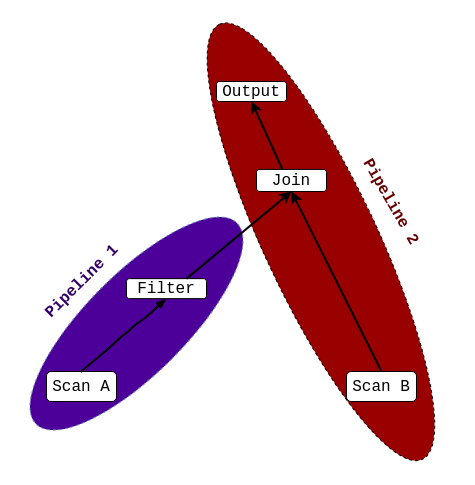
\includegraphics[width=0.9\textwidth]{images/Pipeline.png}
 \caption{Pipelines within the sample query.}
  \label{fig:pipeline_graph}
\end{subfigure}%
\begin{subfigure}{.5\textwidth}
 \centering
 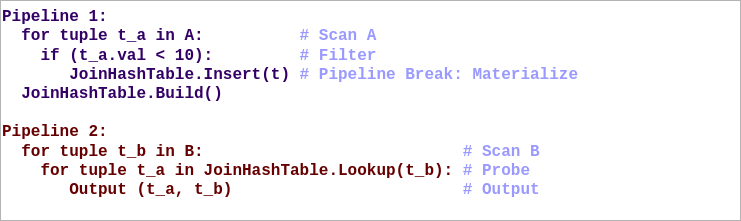
\includegraphics[width=0.9\textwidth]{images/PipelineCode.png}
 \caption{Code generated for the sample query.}
  \label{fig:pipeline_code}
\end{subfigure}
\caption{The compilation model with the sample query. Each pipeline and its corresponding code have the same color.}
\label{fig:update_map_intro}
\end{figure}


Query compilation aims to eliminate the cost of interpretation by compiling the query plan down to machine code.

Talk about related work. (Revise this section).
The data-centric compilation technique pioneered by Hyper \cite{hyper_llvm} splits the plan into several pipelines and compiles them individually. A pipeline is a sequence of relational operators that do not materialize the input result set followed by a pipeline-breaker -- an operator that does materialize the input set (e.g., to build a hash table, or to sort tuples). \cref{fig:pipeline_graph} showcases the pipelines of the sample query. The first pipeline-breaker occurs in the join operator because it needs all input tuples to build a hash table. \cref{fig:pipeline_code} lists the code generated for the query. Conceptually, it performs the same task as \cref{fig:volcano_graph} without any of the virtual function calls. In addition to eliminating interpretation, this approach maximizes register/cache efficiency because a pipeline fully processes a single tuple before fetching the next one. Compilation thus reduces both the number of instructions executed and the number cycles per instructions.

Describe how query compilation works in Noisepage. (Big Picture).

\chapter{Method}

Our proposal is to extend the recovery layer and query compilation layer to support the interpretation of log records. This approach can be realized in three steps:
\begin{enumerate}
\item Extract information from log records.
\item Convert the information into a format that can be accepted and compiled by the code generation engine.
\item Execute the compiled code.
\end{enumerate}

\subsection{Log Record}
The log record structure in Noisepage follows closely to the typical format of a write-ahead log. The header of a log record stores metadata about the log record itself (e.g. record type, record size). The header is then followed by a byte buffer that stores the persisted contents. The size of the byte buffer is also aligned to 8 bytes to ensure the entire log record is aligned to 8 bytes.

During a step of the conventional recovery process, the recovery manager only needs to check the type of the log record and proceed with an insert, update or delete operation. For our method, besides the log record type, we need to find out the contents of the log record as well. This requires additional access to the database catalog.

[Should I expand on the specific types here or later???]
\subsection{Compilation Pipeline}
In Noisepage, a query is first converted into a plan node. The execution engine then translates the plan node into Table Producing Language (TPL) code via a translator object. Finally, the TPL code is compiled into native C++ code. [Also need to explain execution context].

The structure of a log record is different from a query in a number of ways. Firstly, the log record only stores physical information of a committed transaction. For example, an insert query requires the execution engine to retrieve a new tuple slot. For an insert log record, the tuple slot is already been determined and stored within the log record.

These differences require subtle modifications to the compilation process.
Describe Plannodes, Translators that are required for Query Compilation. Can use a graph here.

Describe Execution Context, VM, Bytecode Emitter/Handlers. Interpret vs Compiled.

\subsection{Reinterpreting Log Records}
Describe the process of extracting contents from the log records and converting them into plannodes, translators.

For all records: Find out the mapping from physical column ids to logical column ids.

\subsubsection{Insert Redo Record}
Iterate over the columns of a redo record. Find the value types for each column. Get the value using the previously found value types and column id mappings. Transform each value into an expression value type (ConstantValueExpression/ParameterValueExpression). All the values and metadata are then passed into an Insert Plannode, which is then compiled into an executable query. The tuple slot of the insert operation is retrieved from the execution context, which is then passed to the recovery manager.
\subsubsection{Update Redo Record}
TBD. Should be similar to insert/delete.
\subsubsection{Delete Record}
How to delete index? No information is given on the index, except for the tuple slot to be deleted.

Unless we store a Delta in the delete record, there is no way to get the values.

Pass the delete tuple slot into the execution context, which can be processed in the Bytecode Handler to force the delete operation on the designated tuple slot.

\section{Caching Optimization}
Caching Identifier: Database Oid + Table Oid.
\subsection{Metadata}
Metadata can be cached. Acquire metadata from Catalog. Contents need to be invalidated on drop table?
\subsubsection{Physical to Logical Column Mapping}
Required since the recovery protocol is physical, while query compilation uses logical ids.
\subsubsection{Column Value Types}
This is only for Redo Records. This is required to memcpy the correct values out of a log record into a plan node.
\subsection{Compiled Query}
The compiled query can be cached. Mention that there are two execution modes: Interpret vs Compiled.

For Insert Redo Records: Use ParameterValueExpressions for insert plannodes. Then after compilation, swap in the values to insert into the compiled query into the parameter slots.

For Update Redo Records: ???

For Delete Records: Tuple slot is carried by Execution Context, so not much needs to be done here.
\chapter{Experimental Evaluation}
Mention how the benchmark is implemented.
\section{Throughput Measurement}
Use proper names. Machine specifications. FIO benchmarks. Run experiments with different perspectives.

1. Standard Insert Workload. Single database, single table. 100 percent inserts. Max Columns of 5. 5 statement per txn. Transaction length 5. Allows Varlen.

2. HighStress Insert Workload. Single database, single table. 100 percent inserts. 5 statement per txn. Max Column of 1. Does not allow Varlen.

\chapter{Related Work}
1. A Recovery Algorithm for A High-Performance Memory-Resident Database System. An early paper for disk-based DBMS recovery. Proper log replay infrastructure and checkpoint recoveries. https://15721.courses.cs.cmu.edu/spring2018/papers/12-logging/p104-lehman.pdf

2. Different Logging Schemes. Physical Logging vs Logical Logging. Noisepage uses physical logging. Examples: SiloR (https://15721.courses.cs.cmu.edu/spring2020/papers/10-recovery/zheng-osdi14.pdf). It also uses checkpoints, which does not exist in Noisepage.

3. Different Recovery Schemes. Time-travel table (Azure SQL Database https://15721.courses.cs.cmu.edu/spring2020/papers/10-recovery/p2143-antonopoulos.pdf). Os-fork Snapshots (Hyper, https://dl.acm.org/doi/10.1109/ICDE.2011.5767867)

4. Efficiently Compiling Efficient Query Plans
for Modern Hardware. Early paper abouto query compilation using LLVM framework. https://15721.courses.cs.cmu.edu/spring2020/papers/14-compilation/p539-neumann.pdf

\chapter{Conclusion}

%\appendix
%\include{appendix}

\backmatter

%\renewcommand{\baselinestretch}{1.0}\normalsize

% By default \bibsection is \chapter*, but we really want this to show
% up in the table of contents and pdf bookmarks.
\renewcommand{\bibsection}{\chapter{\bibname}}
%\renewcommand{\bibpreamble}{This text goes between the ``Bibliography''
%  header and the actual list of references}
\bibliographystyle{plainnat}
\bibliography{citations} %your bib file

\end{document}
